\chapter{Valve closing with inlet piping} \label{sec: QWM}

Now, the effect of the fluid within the inlet piping between the pressure tank and pilot-operated PRV will be considered.
First the full system of partial differential equations describing the fluid within the pipework will be considered, which will then be simplified by considering standing acoustic waves.
%Unlike previously in \cref{sec: PDE} where a system of partial differential equations is used to describe the fluid, it is assumed the fluid behaviour is described by a standing quarter acoustic wave.
This method had previously been used to calculate an analytic stability boundary for the simpler direct spring-operated PRV~\cite{Hos2015ModelPipe,Hos2015DynamicModelling,Hos2016DynamicService,Hos2017DynamicRecommendations}. As in \cref{sec: Prog}, the dynamics of the valve will still only be considered while the main valve is closing.

% The pressure and velocity of the fluid within the pipework are functions of time and distance along the pipe. Hence, the fluid properties within the pipe will be described by $p(\eta,t)$ and $v(\eta,t)$ respectively. As before, the fluid is considered only slightly compressible. The slightly compressible nature of the fluid is taken into account while obtaining \cref{eq: FluidPDE}. Hence, the fluid may now be considered incompressible as before, so the density of the fluid is constant. %\textcolor{Red}{REWORD!}

\section{Pipe fluid dynamics}

The fluid within the inlet piping is now a spatio-temporal function. Density, velocity, pressure and internal energy all vary along the length of the pipe and in time. The distance along the pipe will be described by $\eta$, such that $\eta = 0$ at the tank end of the pipe. Hence, the density, velocity, pressure and internal energy distributions will be given by $\rho(\eta,t)$, $v(\eta,t)$, $p(\eta,t)$ and $e(\eta,t)$ respectively.
%Fluid properties such as the pressure, $p(\eta,t)$, and velocity, $v(\eta,t)$, vary along the length of the pipe and in time. The distance along the pipe will be described by $\eta$, such that $\eta = 0$ at the tank end of the pipe.
%\textcolor{Red}{This can be seen in \cref{fig: Diagram}.}
A standard 1D unsteady equation for continuity and conversation of momentum and energy is used to describe the fluid dynamics. These are given by

\begin{equation*}
    \pdiff{}{t} \begin{pmatrix}
    \rho \\ \rho v \\ \rho e
    \end{pmatrix} +
    \pdiff{}{\eta} \begin{pmatrix}
    \rho v \\ \rho v^2 + p \\ \rho v e + p v
    \end{pmatrix} =
    \begin{pmatrix}
    0 \\ \rho \lambda \frac{v \left| v \right|}{2 D} \\ 0
    \end{pmatrix} \, .
\end{equation*}

On the right-hand side of the equation, a non-conservative force represents the frictional loss through the inlet piping, for which $\lambda$ is a friction factor and $D$ is again the diameter of the pipe. However, a number of assumptions will now be made to simplify the partial differential equations describing the fluid.

Firstly, as the working fluid is a liquid, it can be assumed that the temperature of the fluid remains constant as the fluid is almost incompressible. Hence, the energy equation is not required to be considered. Additionally, as the temperature is constant, the density is only a function of the pressure. Hence, $\sfrac{p}{\rho}$ is a conserved quantity. Also, a relationship between the pressure and density can be written in terms of the sonic velocity, $a$, using
~
\begin{equation*}
    \diff{p}{\rho} = a^2 \, .
\end{equation*}

Applying each of these assumptions allows use to simplify the continuity and momentum equations to
~
\begin{equation} \label{eq: FluidPDE}
\begin{split}
    \pdiff{p}{t} + v \pdiff{p}{\eta} + \rho a^2 \pdiff{v}{\eta} &= 0 \\
    \pdiff{v}{t} + v \pdiff{v}{\eta} + \frac{1}{\rho} \pdiff{p}{\eta} &=  \frac{\lambda}{D} v \left| v \right|
\end{split}
\end{equation}

As we may expect, the PDE describing the fluid behaviour is identical to for the direct spring-operated PRV case~\cite{Hos2015ModelPipe}. It is the slight compressibility that allows waves to propagate along the inlet pipe. Now that the slightly compressible nature of the fluid is accounted for while obtaining \cref{eq: FluidPDE}, the fluctuations in density can now be neglected. Hence, the fluid is now considered incompressible as before in \cref{sec: Prog}. Alternatively, the density $\rho$ can be viewed  fluctuating but approximately constant. %\textcolor{Red}{REWORD!}

\subsection{Boundary conditions} \label{subsubsec: BoundCond}

At the valve end of the inlet pipe, $\eta = L$, the velocity is such that mass is conserved between the flow through the pipe and discharged through the main valve. At the tank end of the inlet pipe, $\eta = 0$, the sum of the pressure $p(0,t)$ and the dynamic pressure is equal to the pressure within the tank. This relaxes an assumption made during previous work~\cite{Hos2015ModelPipe}, where the ideal acceleration of the fluid between the tank and the pipe is neglected.

First, considering the boundary condition at $\eta = 0$, the ideal acceleration between the tank and the inlet piping may be written as
~
\begin{equation} \label{eq: QWMBoundary1}
\begin{split}
    p_t(t) &= p(0,t) + \frac{1}{2} \rho(0,t) v(0,t)^2 \\
           &= p_0(t) + \frac{\rho}{2} \left( v_L(t) + C(t) \right)^2 \, .
\end{split}
\end{equation}

Second, the mass conservation at $\eta = L$ imposes the other boundary condition. The mass flow rate at the end of the pipe, when $\eta=L$, is trivially calculated using $\dot{m}(L,t) = \rho A_p v(L,t)$. The discharge from the valve is calculated as before using \cref{eq: ValveMassDischarge}. However, the discharge velocity must be expressed in terms of the pressure and velocity at the end of the pipe. The discharge velocity, $v_d$, can be calculated by considering the conversion of the total pressure into dynamic pressure, rather than the static pressure of the tank in \cref{sec: Prog}. Hence, the second boundary condition can be expressed as
% ADD MORE EXPLANATION OF WHERE THIS EQUATION COMES FROM! Additionally, the mass conservation at $\eta=L$ yields
% %Mass conservation at the outlet of the pipe gives the second boundary condition of
~
\begin{equation*} %\label{eq: QWMBoundary2}
\begin{split}
    \dot{m}(L,t) &= \dot{m}_d(t) \, . \\
    \rho A_p v(L,t) &= \pi D \, x(t) \, C_d \, \rho \sqrt{\frac{2}{\rho} \left( p(L,t) + \frac{\rho}{2} v(L,t)^2 \right)} \, .
\end{split}
\end{equation*}

Here, it is useful to introduce a discharge coefficient, $\zeta = \sqrt{2} \pi D C_d$, to simplify the boundary condition. Hence, the second boundary condition is given by
~
\begin{equation} \label{eq: QWMBoundary2}
    \rho A_p v(L,t) = \zeta \, x(t) \, \sqrt{\rho} \sqrt{ p(L,t) + \frac{\rho}{2} v(L,t)^2 } \, .
\end{equation}

\section{Piston and tank pressure dynamics} \label{subsec: PistonTankDyn}

Now, the dynamics of the main valve piston will be found in terms of the pressure, $p(\eta,t)$, and velocity, $v(\eta,t)$, of the inlet piping fluid. As before in \cref{sec: Prog}, the three forces acting on the piston are the pipe pressure, dome pressure and change of momentum of the fluid. These forces only depend upon the pressure and velocity at the valve end of the pipe, $p(L,t)$ and $v(L,t)$ respectively. Similarly, the differential equation describing the dynamics for the pressure in the tank can be expressed in terms of the same fluid properties, but at the tank end of the pipe, $\eta = 0$. Hence, the differential equations describing the main piston motion and pressure within the tank are given by

\begin{equation} \label{eq: ValveODEsPipe}
\begin{split}
    m_v \ddot{x} + c_v \dot{x} &= A_p p(L,t) - A_v p_t + \dot{m}(L,t)
    %\left(
    v(L,t) %- v_d \sin(\theta) \right)
    \, , \\
    \dot{p}_t &= \frac{a^2}{V} \left( \dot{m}_{in} - \dot{m}(0,t) \right) \, .
\end{split}
\end{equation}

Both these equation depend upon the mass flow rate though the pipe, $\dot{m}(\eta,t)$. Because the fluid is considered incompressible, this can be calculated as the product of the pipe area $A_p$, fluid density $\rho$, and fluid velocity $v(\eta,t)$. Hence, the mass flow rate can be expressed in terms of the velocity using $\dot{m}(\eta,t) = \rho \, A_p \, v(\eta,t)$.

\section{Model reduction}

Now, the pressure and velocity distributions within the pipe will be considered to consist purely of a small amplitude acoustic waves. These distribution occur around the dominant pressure and velocity imposed by the tank pressure and mass discharged through the PRV. It has been shown that the inlet pipe undergoes acoustic waves which are almost identical to those found in an organ pipe~\cite{Botros1997Riser-ReliefInteractions}, where the valve end is considered closed and the tank is an open end. As such, only odd multiples of the quarter-wave frequency satisfy these boundary conditions, so only these need to be considered.
% ~
% \begin{figure}[ht]
%     \centering
%     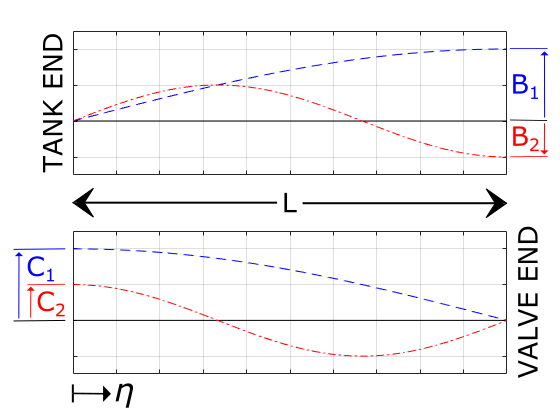
\includegraphics[width=0.7\textwidth]{Diagrams/QWM/QWDiagram.png}
%     \caption{Fluctuations of pressure (top) and velocity (bottom) within the inlet piping.}
%     \label{fig: QWDiagram}
% \end{figure}

During experimental results of chatter, and also for organ-pipe acoustic waves, the velocity oscillations lead the pressure oscillations by $90^o$~\cite{Hos2015DynamicModelling}. Hence, the pressure distribution will be modelled using a $\sin$ function, while the velocity distribution will use a $\cos$ function. A similar approach has previously been adopted for the simpler direct spring-operated PRV \cite{Hos2016DynamicService,Hos2015ModelPipe}. The velocity and pressure distributions of these acoustic waves will be represented by
~
\begin{equation} \label{eq: PressVelDist}
\begin{split}
    p(\eta,t) &= p_0(t) + \sum^{\infty}_{k=1} B_k(t) \, \fun{sin}{2\pi \frac{\eta \left( 2 k - 1 \right)}{4L}} \, ,\\
    v(\eta,t) &= v_L(t) + \sum_{k=1}^{\infty} C_k(t) \, \fun{cos}{2\pi \frac{\eta \left( 2 k - 1 \right)}{4L}} \, .
\end{split}
\end{equation}

\subsection{Galerkin method} \label{subsec: Galerkin}

Now, the fluid dynamical equations from \cref{eq: FluidPDE} will be simplified to a set of ordinary differential equations using the Galerkin method. Only the derivation for pressure fluctuations, $B_k(t)$, will be detailed here. The reader is referred to the appendix for full details of the derivation for $\dot{C}_n$. First, the assumed pressure and velocity distributions from \cref{eq: PressVelDist} are substituted into the mass conservation equation for the fluid piping, \cref{eq: FluidPDE}. This gives the following expression,
~
\begin{equation*}
\begin{split}
    \pdiff{p_0}{t}
    + \sum_{k=1}^{\infty} \dot{B}_k \fun{sin}{2\pi \frac{\eta \left( 2 k - 1 \right)}{4L}}
    + v_L \sum_{k=1}^{\infty} B_k \frac{\pi \left( 2 k - 1 \right)}{2L} \fun{cos}{2\pi \frac{\eta \left( 2 k - 1 \right)}{4L}} 
    & \\ % newline
    + \sum_{k=1}^{\infty} \sum_{m=1}^{\infty} C_k B_m \frac{\pi \left( 2 m - 1 \right)}{2L} \fun{cos}{2\pi \frac{\eta \left( 2 k - 1 \right)}{4L}} \fun{cos}{2\pi \frac{\eta \left( 2 m - 1 \right)}{4L}} 
    & \\ % newline
    - \rho a^2 \sum_{k=1}^{\infty} C_k \frac{\pi \left( 2 k - 1 \right)}{2L} \fun{cos}{2\pi \frac{\eta \left( 2 k - 1 \right)}{4L}}
    &= 0 \, .
\end{split}
\end{equation*}

% \begin{equation*}
% \begin{split}
%     \dot{v}_L
%     + \sum_{k=1}^{\infty} \dot{C}_k \fun{cos}{2\pi \frac{\eta \left( 2 k - 1 \right)}{4L}}
%     - v_L \sum_{k=1}^{\infty} C_k \frac{\pi \left( 2 k - 1 \right)}{2L} \fun{sin}{2\pi \frac{\eta \left( 2 k - 1 \right)}{4L}}
%     & \\ % newline
%     - \sum_{k=1}^{\infty} \sum_{m=1}^{\infty} C_k C_m \frac{\pi \left( 2 m - 1 \right)}{2L} \fun{cos}{2\pi \frac{\eta \left( 2 k - 1 \right)}{4L}} \fun{sin}{2\pi \frac{\eta \left( 2 m - 1 \right)}{4L}} 
%     & \\ % newline
%     + \frac{1}{\rho} \sum_{k=1}^{\infty} B_k \frac{\pi \left( 2 k - 1 \right)}{2L} \fun{cos}{2\pi \frac{\eta \left( 2 k - 1 \right)}{4L}}
%     &= \\ % newline
%     \frac{\lambda}{D} \left( v_L + \sum_{k=1}^{\infty} C_k \fun{cos}{2\pi \frac{\eta \left( 2 k - 1 \right)}{4L}} \right) \left| v_L + \sum_{k=1}^{\infty} C_k \fun{cos}{2\pi \frac{\eta \left( 2 k - 1 \right)}{4L}} \right|
% \end{split}
% \end{equation*}

Notice that the dynamics of all modes are coupled, as $\dot{B}_k$ appears for each of the $k$ modes. The Galerkin method uses the orthogonality between each mode to isolate an ordinary differential equation for an arbitrary mode, $B_n$. Hence, the equations above are multiplied by the arbitrary mode-shape, $\sin\left(2\pi\frac{\eta(2k-1)}{4L}\right)$ and then integrated over the domain of interest, from $0$ to $L$. Doing so gives
~
\begin{equation*}
\begin{split}
    \pdiff{p_0}{t} \int^L_0 \sin\left(2\pi\frac{\eta(2n-1)}{4L}\right) \Idx{\eta}
    + \sum_{k=1}^{\infty} \dot{B}_k \int^L_0 \fun{sin}{2\pi \frac{\eta \left( 2 k - 1 \right)}{4L}} \sin\left(2\pi\frac{\eta(2n-1)}{4L}\right) \Idx{\eta}
    & \\ % newline
    + v_L \sum_{k=1}^{\infty} B_k \frac{\pi \left( 2 k - 1 \right)}{2L} \int^L_0 \fun{cos}{2\pi \frac{\eta \left( 2 k - 1 \right)}{4L}} \sin\left(2\pi\frac{\eta(2n-1)}{4L}\right) \Idx{\eta}
    & \\ % newline
    + \sum_{k=1}^{\infty} \sum_{m=1}^{\infty} C_k B_m \frac{\pi \left( 2 m - 1 \right)}{2L} \int^L_0 \fun{cos}{2\pi \frac{\eta \left( 2 k - 1 \right)}{4L}} \fun{cos}{2\pi \frac{\eta \left( 2 m - 1 \right)}{4L}} \sin\left(2\pi\frac{\eta(2n-1)}{4L}\right) \Idx{\eta}
    & \\ % newline
    - \rho a^2 \sum_{k=1}^{\infty} C_k \frac{\pi \left( 2 k - 1 \right)}{2L} \int^L_0 \fun{cos}{2\pi \frac{\eta \left( 2 k - 1 \right)}{4L}} \sin\left(2\pi\frac{\eta(2n-1)}{4L}\right) \Idx{\eta}
    &= 0 \, .
\end{split}
\end{equation*}

The orthogonality conditions then mean that the only derivative with non-zero coefficient is $\dot{B}_n$. Hence, a separate equation for each temporal derivatives for the pressure fluctuation amplitudes can be found. Applying the orthogonality conditions and evaluating the remaining integrals give the generalised equation for $\dot{B}_n(t)$ as
~
\begin{equation*}
\begin{split}
    \dot{B}_n &=
    \rho a^2 \frac{(2n-1)\pi}{2L} C_n
    - \frac{4}{\pi(2n-1)} \pdiff{p_0}{t}
    - \frac{1}{L} v_L \left( B_n + \sum^{\infty}_{k = 1,n \neq k} \frac{2k-1}{n-k} B_k \right)
    \\ & \quad
    - \frac{2}{L} \sum^{\infty}_{k=1} \sum^{\infty}_{m=1} C_k B_m \frac{
    (2m-1)(1-2n)(4k^2 - 4k + 4m^2 - 4m - 4n^2 + 4n + 1)
    }{
    (2(k+m+n)-3)(2(k-m+n)-1)(2(k+m-n)-1)(2(k-m-n)+1)
    } \, .
\end{split}
\end{equation*}

% Similarly for $\dot{C}_n$, multiplying by the shape function and integrating over the domain gives
% ~
% \begin{equation*}
% \begin{split}
%     \dot{v}_L \int^L_0 \cos\left(2\pi\frac{\eta(2n-1)}{4L}\right) \Idx{\eta}
%     + \sum_{k=1}^{\infty} \dot{C}_k \int^L_0 \fun{cos}{2\pi \frac{\eta \left( 2 k - 1 \right)}{4L}} \cos\left(2\pi\frac{\eta(2n-1)}{4L}\right) \Idx{\eta}
%     & \\ % newline
%     - v_L \sum_{k=1}^{\infty} C_k \frac{\pi \left( 2 k - 1 \right)}{2L} \int^L_0 \fun{sin}{2\pi \frac{\eta \left( 2 k - 1 \right)}{4L}} \cos\left(2\pi\frac{\eta(2n-1)}{4L}\right) \Idx{\eta}
%     & \\ % newline
%     - \sum_{k=1}^{\infty} \sum_{m=1}^{\infty} C_k C_m \frac{\pi \left( 2 m - 1 \right)}{2L} \int^L_0 \fun{cos}{2\pi \frac{\eta \left( 2 k - 1 \right)}{4L}} \fun{sin}{2\pi \frac{\eta \left( 2 m - 1 \right)}{4L}} \cos\left(2\pi\frac{\eta(2n-1)}{4L}\right) \Idx{\eta}
%     & \\ % newline
%     + \frac{1}{\rho} \sum_{k=1}^{\infty} B_k \frac{\pi \left( 2 k - 1 \right)}{2L} \int^L_0 \fun{cos}{2\pi \frac{\eta \left( 2 k - 1 \right)}{4L}} \cos\left(2\pi\frac{\eta(2n-1)}{4L}\right) \Idx{\eta}
%     &= \\ % newline
%     \frac{\lambda}{D} \int^L_0 \left( v_L + \sum_{k=1}^{\infty} C_k \fun{cos}{2\pi \frac{\eta \left( 2 k - 1 \right)}{4L}} \right) \left| v_L + \sum_{k=1}^{\infty} C_k \fun{cos}{2\pi \frac{\eta \left( 2 k - 1 \right)}{4L}} \right| \cos\left(2\pi\frac{\eta(2n-1)}{4L}\right) \Idx{\eta}
% \end{split}
% \end{equation*}

As previously mentioned, the derivation for $\dot{C}_n(t)$ is omitted here as is the same steps applied to the momentum equation. Again, the reader is referred to the appendix for full details of the derivation. After using the Galerkin method on the momentum equation, the generalised equation for $\dot{C}_n(t)$ is
~ 
\begin{equation*}
\begin{split}
    \dot{C}_n &=
    \frac{4}{\pi} \frac{(-1)^n}{2n-1} \pdiff{v_L}{t}
    + \frac{1}{L} v_L \sum^{\infty}_{k=1,k \neq n} C_k \frac{2k-1}{k-n}
    + \frac{1}{L} v_L C_n
    - \frac{1}{\rho} \sum^{\infty}_{k=1} B_k \frac{\pi (2k-1)}{2L}
    \\ & \quad % newline
    - \frac{2}{L} \sum^{\infty}_{k=1} \sum^{\infty}_{m=1} C_k C_m \frac{
    (2m-1)^2 (4k^2 - 4k + 4m^2 - 4m - 4n^2 + 4n + 1)
    }{
    (2(k+m+n)-3)(2(k-m+n)-1)(2(k+m-n)-1)(2(k-m-n)+1)
    }
    \\ & \quad % newline
    - \frac{\lambda}{D} \frac{4}{\pi} \frac{(-1)^n}{2n-1} v_L\power{2}
    + 2 \frac{\lambda}{D} v_L C_n
    \\ & \quad % newline
    + \frac{\lambda}{D} \frac{8}{\pi} \sum^{\infty}_{k=1} \sum^{\infty}_{k=1} C_k C_m \frac{
    (-1)^k (-1)^m (-1)^n (2k-1) (2m-1) (2n-1)
    }{
    (2(k+m+n)-3)(2(k-m+n)-1)(2(k+m-n)-1)(2(k-m-n)+1)
    } \, .
\end{split}
\end{equation*}

Obviously, it is impossible to consider the infinite number of modes considered by $k \in [1,\infty]$. Instead, an approximation by taking only a finite number of modes is used. As the one-mode truncation was found appropriate for the spring-operated case~\cite{Hos2015ModelPipe}, a one-mode truncation will be used here. Hence, the ordinary differential equations describing the quarter-wave are given by
~
\begin{equation*}
\begin{split}
    \dot{B}_1 &= \rho a^2 \frac{\pi}{2 L} C_1 - \frac{4}{\pi} \pdiff{p_0}{t} - \frac{1}{L} v_L B_1 - \frac{2}{3L} C_1 B_1 \, ,
    \\
    \dot{C}_1 &= - \frac{4}{\pi} \pdiff{v_L}{t} + \frac{1}{L} v_L C_1 - \frac{1}{\rho} \frac{\pi}{2L} B_1 + \frac{2}{3L} C_1\power{2} + \frac{\lambda}{D} \frac{4}{\pi} v_L\power{2} + 2 \frac{\lambda}{D} v_L C_1 + \frac{\lambda}{D} \frac{8}{3 \pi} C_1\power{2} \, .
\end{split}
\end{equation*}

\subsection{Collocation technique}

An alternative approach for reducing the partial differential equation given in \cref{eq: FluidPDE} to a system of ordinary differential equations is the collocation technique. Instead of considering the entire length of the pipe, the collocation technique ensure the partial differential equation is satisfied at a number of points along the pipe. It is more difficult to use the collocation technique for the general case of $N$ nodes, so a one-mode truncation will immediately be used. Hence, the subscripts will be dropped so $B_1 = B$ and $C_1 = C$. As the one-mode truncation is used, the fluid equations must only be satisfied at a single location, chosen as the mid-point of the pipe where $\eta = \frac{L}{2}$.
%
At this point, $\fun{sin}{2 \pi \frac{\eta}{4L}} = \fun{cos}{2 \pi \frac{\eta}{4L}} = \frac{1}{\sqrt{2}}$.
%
The pressure and velocity distributions from \cref{eq: PressVelDist} are substituted into the fluid PDEs from \cref{eq: FluidPDE}. Considering that $\eta = \frac{L}{2}$, and rationalising by multiplying by $\sqrt{2}$, requires that
~
\begin{equation} \label{eq: CollocationODE}
\begin{split}
    \sqrt{2} \dot{p}_0(t) + \dot{B}(t) + \frac{\pi \sqrt{2}}{4 L} B(t) \left( \sqrt{2} v_L(t) + C(t) \right) &= a^2 \rho \frac{\pi}{2L} C(t) \, , \\
    \sqrt{2} \dot{v}_L(t) + \dot{C}(t) - \frac{\pi \sqrt{2}}{4 L} C(t) \left( \sqrt{2} v_L(t) + C(t) \right) &= - \frac{1}{\rho} \frac{\pi}{2 L} B(t) \\
    &\qquad + \frac{\lambda \sqrt{2}}{2D} \left( \sqrt{2} v_L(t) + C(t) \right) \left| \sqrt{2} v_L(t) + C(t) \right| \, .
\end{split}
\end{equation}

\subsection{Comparison of model reductions}

Now, a comparison between the coefficients for each of the terms of the ordinary differential equations derived by the Galerkin and Collocation techniques. \Cref{tab: GalerkinCollocationComparison} lists each of the coefficients which were calculated by the two different methods. Clearly, all the coefficients are of the same order of magnitude, and most have a relatively small error between them.

\begin{table}[ht]
    \centering \renewcommand*{\arraystretch}{1.4}
    \begin{tabular}{c|c ?{0.5mm} c|c ?{0.5mm} c}
        \multicolumn{2}{c ?{0.5mm} }{Galerkin} & \multicolumn{2}{c ?{0.5mm} }{Collocation} & \\ \cline{1-4}
        Exact & Decimal & Exact & Decimal & Error \\ \hline \hline
        $\frac{4}{\pi}$ & $1.2732$ & $\sqrt{2}$ & $ 1.4142 $ & $ 10.0\% $ \\[2pt] \hline
        $1$ & $1.0000$ & $\frac{\pi}{2}$ & $1.5708$ & $36.3\%$ \\[2pt] \hline
        $\frac{2}{3}$ & $0.6667$ & $\frac{\pi \sqrt{2}}{4}$ & $1.1107$ & $40.0\%$ \\[2pt] \hline
        $\frac{\pi}{2}$ & $1.5708$ & $\frac{\pi}{2}$ & $1.5708$ & $0\%$ \\[2pt] \hline
        $2$ & $2.0000$ & $2$ & $2.0000$ & $0\%$ \\  \hline
        $\frac{8}{3 \pi}$ & $0.8488$ & $\frac{\sqrt{2}}{2}$ & $0.7071$ & $16.7\%$
    \end{tabular}
    \caption{Comparison of the different coefficients found for the quarter-wave model using the Galerkin and Collocation techniques.}
    \label{tab: GalerkinCollocationComparison}
\end{table}

However, two of the coefficients have a error between them of $36.3\%$ and $40.0\%$. Both of these coefficients are from the convective terms of the partial differential equation, which are generally negligible for the compressible liquid case~\cite{Hos2016DynamicService}. That the convective effects are negligible will confirmed in \cref{subsec: QWMNonDim} when the dimensionless differential equations are calculated. Hence, the difference between using the Galerkin and Collocation techniques appears largely unimportant.

\section{Quarter-wave derivation} \label{subsec: QWM Derivation}

As stated previously, the one-mode truncation was found appropriate for the spring-operated case~\cite{Hos2015ModelPipe}. Therefore, one the one-mode truncation will now be considered, corresponding to the acoustic quarter-wave. For a direct spring-operated PRV, using the Collocation technique to perform a model reduction was shown to be quantitatively similiar to experimental data~\cite{Hos2015DynamicModelling}. Hence, only the coefficients from the Collocation technique will be used, which also ensures the following analysis is consistent with the spring-operated case. We begin by ensuring the boundary conditions are satisfied by the quarter-wave model.
%
%\subsection{Boundary conditions}

Unfortunately, fully satisfying the boundary conditions defined by \cref{eq: QWMBoundary1,eq: QWMBoundary2} yields complicated expressions for $p_0(t)$ and $v_L(t)$.
% The velocity at the end of the pipe is given by
% ~
% \begin{equation*}
%     v_L(t) = \frac{1}{2} \left( \frac{\zeta x}{A_p \sqrt{\rho}} \right)^2 \left( - \rho C(t) + \sqrt{4 \left( \frac{A_p \sqrt{\rho}}{\zeta x} \right)^2 \left( p_t(t) + B(t) \right) + \rho^2 C(t)^2 \left( 1 - 2 \frac{A_p\power{2}}{\zeta^2 x^2} \right)} \, \right) \, .
% \end{equation*}
% 
% As $C(t)$ is a small fluctuation, a binomial expansion may be applied to the square-root term, to give
% ~
% \begin{equation*}
%     v_L(t) = \frac{\zeta x}{A_p \sqrt{\rho}} \sqrt{p_t(t) + B(t)} - 
%     \left( \frac{\zeta x}{A_p \sqrt{\rho}} \right)^2 \left( \frac{1}{2} \rho C(t) - \frac{1}{8} \frac{\zeta x}{A_p \sqrt{\rho}} \frac{\rho^2 C(t)^2}{\sqrt{p_t(t) + B(t)}} \left( 1 - 2 \frac{A_p\power{2}}{\zeta^2 x^2} \right) \right) \, .
% \end{equation*}
Additionally, both the pressure and velocity distributions, $p(\eta,t)$ and $v(\eta,t)$, are functions of both $B$ and $C$. Therefore, when $\pdiff{p}{t}$ and $\pdiff{v}{t}$ to ensure \cref{eq: FluidPDE} is satisfied, each of two ordinary differential equations contains $\dot{B}$ and $\dot{C}$.
%However, as both $p(\eta,t)$ and $v(\eta,t)$ are functions of $B$ and $C$, both ordinary differential equations are in terms of $\dot{B}$ and $\dot{C}$.
As the system is linear for $\dot{B}$ and $\dot{C}$, the set of differential equation could be solved, but involves algebra too long to be of use for further analysis.

%\newpage
The most general simplification is to neglect the fluctuations in velocity, $C(t) \approx 0$, when calculating the boundary condition given by \cref{eq: QWMBoundary1}. As $C(t)$ represents a small amplitude oscillation, the assumption that $v_L(t) + C(t) \approx v_L(t)$ is valid.
%However, if large amplitude oscillations occur, then the boundary conditions will no longer be satisfied.
As this model is only interested in the onset of a flutter instability, this is an acceptable assumption. Using this assumption, the boundary conditions can be solved to give
~
\begin{equation} \label{eq: QWMPresAndVelBound}
    p_0(t) = p_t(t) - \frac{\zeta^2 x^2}{2 A_p\power{2}} \left( p_t(t) \textcolor{Red}{+ B(t)} \right)
    \, , \qquad
    v_L(t) = \frac{\zeta x}{A_p \sqrt{\rho}} \sqrt{p_t(t) + B(t)} \, .
\end{equation}

The expression for $v_L(t)$ is identical to that for the direct spring-operated case~\cite{Hos2015ModelPipe}, but $p_0(t) \neq p_t(t)$ because the conversion of the tank static pressure into dynamic pressure is considered as discussed in \cref{subsubsec: BoundCond}. Another small fluctuation for which it may be possible to ignore using a similar argument to $C(t)$ is shown in \textcolor{Red}{red}. For completeness, this \textcolor{Red}{red} term will initially not be neglected, with \textcolor{Red}{red} terms in later equations indicating that those terms occur from considering the small fluctuation, $\textcolor{Red}{B(t)}$.
%
%\subsection{Piston and tank pressure dynamics}

Now that the values of $p_0(t)$ and $v_L(t)$ have been found, the pressure and velocity distributions from \cref{eq: PressVelDist,eq: QWMPresAndVelBound} can be substituted into the previous equations of motion for the valve and tank pressure found in \cref{subsec: PistonTankDyn}. Using the previous results, \cref{eq: ValveODEsPipe} becomes
~
\begin{equation*}
\begin{split}
    m_v \ddot{x} + c_v \dot{x} &= \frac{\zeta^2 x^2}{2 A_p} p_t(t) + \frac{\zeta^2 x^2}{A_p} \left( 1 \textcolor{Red}{- \frac{1}{2}} \right) B(t) - \left( A_v - A_p \right) p_t(t)
    \, , \\
    \dot{p}_t &= \frac{a^2}{V} \left( \dot{m}_{in} - \rho A_p C(t) - \zeta x(t) \sqrt{\rho} \sqrt{p_t(t) + B(t)} \right) \, .
\end{split}
\end{equation*}

With zero amplitude of the quarter wave, so $B(t) = C(t) = 0$, the equations reduce to the original equations for the valve closing model, \cref{eq: ClosingDiffEqFull}, presented in \cref{sec: Prog}. However, if the ideal acceleration of the fluid for the boundary condition \cref{eq: QWMBoundary1}, then the equation of motion is not identical to previously. The force acting on the main piston due to the change in momentum is counteracted by the decrease in fluid static pressure due to the fluid flow. Neglecting the conversion between dynamic and static conversion would overestimate the force acting on the valve by a factor of two.
%
%\subsection{Quarter wave fluid equations} 

Finally, the differential equation for both $\dot{B}(t)$ and $\dot{C}(t)$ must be found. The first equation found by the collocation technique can be re-arranged to find an expression for $\dot{B}(t)$. Substituting the expressions for $p_0(t)$ and $v_L(t)$ into \cref{eq: CollocationODE} gives
~
%EQUATION FOR $\dot{B}(t)$.
\begin{equation}  \label{eq: QWMFullDiffB}
\begin{split}
    \dot{B}(t) = \left( \frac{2 A_p\power{2}}{2 A_p\power{2} \textcolor{Red}{- \sqrt{2} \zeta^2 x(t)^2}} \right)
    &\left( \textcolor{Blue}{
    \frac{\pi}{2L} a^2 \rho C(t) - \frac{\pi \sqrt{2}}{4L} \left( \sqrt{2} v_L(t) + C(t) \right) - \sqrt{2} \dot{p}_t(t)}
     \right.  \\ & \quad \left.  % linebreak
    + \frac{\sqrt{2} \zeta^2 x(t)^2}{2 A_p\power{2}} \dot{p}_t(t) + \frac{\sqrt{2} \zeta^2 x(t)}{A_p\power{2}} \left( p_t(t) \textcolor{Red}{+ B(t)} \right) \dot{x}(t)
    \right) \, .
\end{split}
\end{equation}

As previously noted, \textcolor{Red}{red} terms will not appear if the small amplitude oscillation \textcolor{Red}{$B(t)$} is neglected. Consider the case when \textcolor{Red}{$B(t)$} is neglected. Terms which are coloured \textcolor{Blue}{blue} occur within the derivation of a QWM for a spring-operated PRV~\cite{Hos2015ModelPipe}. Therefore, it is seen that some additional higher order terms which appear as those coloured in black. These higher order terms occur by considering of the ideal acceleration between the tank and inlet piping as discussed in \cref{subsubsec: BoundCond}.

%%%%%%%%%%%%%%%%%%%%
%% GOT UP TO HERE %%
%%%%%%%%%%%%%%%%%%%%
Similarly, the second equation calculated from Collocation technique may be re-arranged to find an ordinary differential equation for $\dot{C}(t)$. The terms will be coloured in the same way as \cref{eq: QWMFullDiffB}. However, unlike for $\dot{B}(t)$, the equation for $\dot{C}(t)$ also contains $\dot{B}(t)$, which when substituted in gives
% The terms are coloured in the same way as before. Notably, the equation for $\dot{C}(t)$ is a function of $\dot{B}(t)$. This contributes to the long and unwieldy equation above which is difficult to manipulate algebraically.
~
\begin{equation} \label{eq: QWMFullDiffC}
\begin{split}
    \dot{C}(t) &=
    \textcolor{Blue}{
    \frac{\pi}{2L} \frac{\zeta}{A_p \sqrt{\rho}} x C \sqrt{p_t + B}
    + \frac{\pi \sqrt{2}}{4 L} C^2
    - \frac{1}{\rho} \frac{\pi}{2L} B
    } \\ & \quad % linebreak
    - \frac{\sqrt{2} \zeta}{2 A_p \sqrt{\rho}} \frac{1}{\sqrt{p_t+B}} \left( \frac{2 A_p\power{2}}{2 A_p\power{2} \textcolor{Red}{- \sqrt{2} \zeta^2 x^2}} \right) x \left(
    \textcolor{Blue}{
    \frac{\pi}{2L} a^2 \rho C
    - \frac{\pi \sqrt{2}}{4 L} B C
    - \frac{\pi}{2L} B v_L }
    \right)
    \\ & \quad % linebreak
    - \frac{\zeta}{A_p \sqrt{\rho}} \dot{x} \sqrt{p_t + B} \left( 
    \frac{ 2 \sqrt{2} \left( p_t + B \right) A_p\power{2} + 2 \zeta^2 x^2 \left( p_t \textcolor{red}{+ B} \right) \textcolor{Red}{- 2 \zeta^2 x^2 \left( p_t + B \right)} }
    { \left( p_t + B \right) \left( 2 A_p\power{2} \textcolor{Red}{- \sqrt{2} \zeta^2 x^2} \right) }
    \right)
    \\ & \quad % linebreak
    + \frac{\zeta}{A_p \sqrt{\rho}} \frac{x \dot{p}_t}{\sqrt{p_t+B}} \left( \frac{
    \textcolor{Blue}{\left( 2 - \sqrt{2} \right) A_p\power{2}}
    - \zeta^2 x^2 \textcolor{Red}{+ \zeta^2 x^2}}{
    \textcolor{Blue}{2 A_p\power{2}}
    \textcolor{Red}{+ \sqrt{2} \zeta^2 x^2}} \right)
    \\ & \quad % linebreak
    \textcolor{Blue}{
    + \frac{\lambda \sqrt{2}}{4 D} \left( \sqrt{2} v_L + C \right) \left| \sqrt{2} v_L + C \right| } \, .
\end{split}
\end{equation}

% \section{Actual pressure and velocity profiles}

% Neglecting the small change in velocity at the tank end of the inlet piping. The pressure and velocity distributions are:

% \begin{equation} \label{eq: BetterPressVelDist}
% \begin{split}
%     p(\eta,t) &= p_t(t) - \frac{\zeta^2 x^2}{2 A_p\,^2} \left( p_t(t) + B(t) \right) + B(t) \fun{sin}{2\pi \frac{\eta}{4L}} \, ,\\
%     v(\eta,t) &= v_L(t) + C(t) \fun{cos}{2\pi \frac{\eta}{4L}} \, .
% \end{split}
% \end{equation}

% Substituting these distributions into equations of motion of valve and tank pressure yields:

% \begin{equation*}
% \begin{split}
%     m_v \ddot{x} + c_v \dot{x} &= A_p \left( 1 - \frac{\zeta^2 x^2}{2 A_p\,^2} \right) \left( p_t(t) + B(t) \right)  - A_v p_t + \rho A_p %v(L,t)^2
%     \left( \frac{\zeta x}{A_p \sqrt{\rho}} \sqrt{p_t(t) + B(t)} \right)^2 \\
%     \dot{p}_t %&= \frac{a^2}{V} \left( \dot{m}_{in} - \dot{m}(0,t) \right)
%     &= \frac{a^2}{V} \left( \dot{m}_{in} - \zeta x \sqrt{\rho} \sqrt{p_t(t) + B(t)} - \rho A_p C(t) \right)
% \end{split}
% \end{equation*}

%\newpage
%% At the inlet of the pipe, an ideal inflow from the tank using Bernoulli's equation allows the first boundary condition

% \begin{equation*}
%     p_t(t) = p(0,t) + \frac{1}{2} \rho(0,t) v(0,t)^2
% \end{equation*}

% Mass conservation at the outlet of the pipe gives the second boundary condition of

% \begin{equation*}
%     \dot{m}(L,t) = \rho(L,t) A_p v(L,t) = \dot{m}_d(t)
% \end{equation*}

The assumed velocity and pressure distributions are a quarter-wave of the inlet pipe, given by
~
\begin{equation} %\label{eq: PressVelDist}
\begin{split}
    p(\eta,t) &= p_t(t) + B(t) \fun{sin}{2\pi \frac{\eta}{4L}} \, ,\\
    v(\eta,t) &= v_L(t) + C(t) \fun{cos}{2\pi \frac{\eta}{4L}} \, .
\end{split}
\end{equation}

These distributions fulfil the boundary conditions of equalling the tank pressure ($p_t(t)$) at $\eta = 0$ and mass conservation with the discharge at $\eta = L$. Here, the velocity at $\eta = L$ is
~
\begin{equation*}
    v_L(t) = \frac{\sqrt{2} \pi D C_d}{A_p \sqrt{\rho}} x(t) \sqrt{p_t(t)+B(t)} \, .
\end{equation*}

Substituting the velocity and pressure distributions given by \cref{eq: PressVelDist} into the PDE describing the fluid flow (\cref{eq: FluidPDE}) gives a differential equation which must be satisfied at all locations along the pipe. Using the collocation technique, it is sufficient that this differential equation is only satisfied at the mid-point of the pipe, where $\eta = \frac{L}{2}$. Here, $\fun{sin}{2 \pi \frac{\eta}{4L}} = \fun{cos}{2 \pi \frac{\eta}{4L}} = \frac{1}{\sqrt{2}}$. This requires that
~
\begin{equation*}
\begin{split}
    \sqrt{2} \dot{p}_t(t) + \dot{B}(t) + \frac{\pi \sqrt{2}}{4 L} B(t) \left( \sqrt{2} v_L(t) + C(t) \right) &= a^2 \rho \frac{\pi}{2L} C(t) \, , \\
    \sqrt{2} \dot{v}_L(t) + \dot{C}(t) - \frac{\pi \sqrt{2}}{4 L} C(t) \left( \sqrt{2} v_L(t) + C(t) \right) &= - \frac{1}{\rho} \frac{\pi \sqrt{2}}{2 L} B(t) \\
    &\qquad + \lambda \frac{L}{2D} \left( \sqrt{2} v_L(t) + C(t) \right) \left| \sqrt{2} v_L(t) + C(t) \right| \, .
\end{split}
\end{equation*}

Note that these two equations form a set of differential equations for $\dot{B}(t)$ and $\dot{C}(t)$, which can be added to the original three first order differential equations describing the motion of the valve and pressure in the tank. Also note the last term including $\lambda$ is a frictional loss through the pipe, which may initially be neglected. Also, $\dot{v}_L(t)$ is used instead of the lengthy expression, which is
~
\begin{equation*}
    \dot{v}_L(t) = \frac{\sqrt{2} \pi D C_d}{A_p \sqrt{\rho}} \sqrt{p_t(t) + B(t)} \left( \dot{x}(t) + \frac{1}{2} x(t) \frac{\dot{p}_t(t) + \dot{B}(t)}{p_t(t) + B(t)} \right) \, .
\end{equation*}

The differential equation describing the tank pressure, using the assumed velocity distribution, can be written as
~
\begin{equation*}
    \dot{p}_t(t) = \frac{a^2}{V} \left( \dot{m}_{in} - \rho A_p C(t) - \sqrt{2} \pi D C_d x(t) \sqrt{\rho} \sqrt{p_t(t) + B(t)} \right) \, .
\end{equation*}

The full set of differential equations are
~
\begin{equation*}
\begin{split}
    \dot{x} &= v \\
    \dot{v} &= - \frac{c_v}{m_v} v + \frac{A_p}{m_v} B + \frac{\zeta^2}{m_v A_p} x^2 B + \frac{\zeta^2}{m_v A_p} x^2 p_t - \frac{A_v - A_p}{m_v} p_t \\
    \dot{p}_t &= \frac{a^2}{V} \left( \dot{m}_{in} - \rho A_p C(t) - \sqrt{2} \pi D C_d x(t) \sqrt{\rho} \sqrt{p_t(t) + B(t)} \right) \, , \\
    \dot{B} &= a^2 \rho \frac{\pi}{2L} C - \sqrt{2} \dot{p}_t - \frac{\pi}{2L} \frac{\sqrt{2} \pi D C_d}{A_p \sqrt{\rho}} x B \sqrt{p_t + B} - \frac{\pi \sqrt{2}}{4L} B C \, , \\
    ~
    \dot{C} &=
    \frac{\pi \zeta}{2 A_p L \sqrt{\rho}} x C \sqrt{p_t + B}
    + \frac{\pi \sqrt{2}}{4L} C^2
    - \frac{\pi}{2 L \rho} B
    - \frac{\sqrt{2} \zeta}{A_p \sqrt{\rho}} v \sqrt{p_t + B}
    + \frac{2 - \sqrt{2}}{2} \frac{\zeta}{A_p \sqrt{\rho}} \frac{x}{\sqrt{p_t + B}} \dot{p}_t \\ &\quad %linebreak
    - \frac{\sqrt{2}\pi\zeta a^2 \rho}{4 L A_p \sqrt{\rho}} \frac{x C}{\sqrt{p_t + B}}
    + \frac{\sqrt{2}\pi\zeta^2}{4L A_p\,^2 \rho} x^2 B
    + \frac{\pi \zeta}{4 L A_p \sqrt{\rho}} \frac{x B C}{\sqrt{p_t + B}}
    + \lambda \frac{\sqrt{2}L}{4 D} \left( \sqrt{2} v_L + C \right) \left| \sqrt{2} v_L + C \right|
\end{split}
\end{equation*}

where $\zeta = \sqrt{2} \pi D C_d$.

\section{Final reduced equations} \label{subsec: QWMFinalDimensional}

% Explain why neglected \textcolor{Red}{B(t)} term
% Write out full set of 5 ODEs

Because of the lengthy and unwieldy expression for $\dot{C}(t)$, the \textcolor{Red}{$B(t)$} will be neglected. Neglecting this small pressure fluctuation is in a similar way to how the dynamic pressure at the tank end of the pipe was previously approximated using $v(0,t) = v_L(t) + C(t) \approx v_L(t)$ in \cref{eq: QWMBoundary1}. Hence, the dynamic pressure is $p_t(t) + B(t) \approx p_t(t)$. This simplifies the ordinary differential equations given by \cref{eq: QWMFullDiffB,eq: QWMFullDiffC} by removing any terms coloured in \textcolor{Red}{red}. This may also be seen as ensuring the boundary conditions, \cref{eq: QWMBoundary1,eq: QWMBoundary2}, are fully satisfied when the quarter-wave does not occur so $B(t) = C(t) = 0$. This assumption is reasonable as the quarter-wave model aims to study the system close to the onset of a flutter instability, at which both $B(t)$ and $C(t)$ will be close to zero.

An additional bonus of using this simplification is the differential equations are consistent with those previously derived for a quarter-wave model in the liquid case, for example in~\cite{Hos2015ModelPipe}. The expression for $v_L$ given previously in \cref{eq: QWMPresAndVelBound} will be used to write the quarter-wave model more compactly. The terms which are coloured in \textcolor{Blue}{blue} in \cref{eq: FullQWMDimensional} represent those which occur for the spring-operated case. Again, the differences appear from considering the ideal acceleration of the fluid between the tank and the pipe when considering the boundary condition, \cref{eq: QWMBoundary1}. These differences always appear as higher-order terms seen in black, which include the ratio between the discharge area, $\zeta x$, and the pipe area, $A_p$. This ratio will later be shown as an important parameter for the pilot-operated PRV. The full set of five first-order differential equations, which will be referred to as the quarter-wave model, are given by
~
\begin{equation} \label{eq: FullQWMDimensional}
\begin{split}
    \dot{x} &= v \, , \\
    m_v \dot{v} &= - c_v v + \frac{\zeta^2 x^2}{2 A_p} p_t(t) + \frac{\zeta^2 x^2}{A_p} B(t) - \left( A_v - A_p \right) p_t(t)
    \, , \\
    \dot{p}_t &= \frac{a^2}{V} \left( \dot{m}_{in} - \rho A_p C(t) - \zeta x(t) \sqrt{\rho} \sqrt{p_t(t) + B(t)} \right)
    \, , \\
    \dot{B}(t) &= \textcolor{Blue}{
    \frac{\pi}{2L} a^2 \rho C(t) - \frac{\pi \sqrt{2}}{4L} \left( \sqrt{2} v_L(t) + C(t) \right) - \sqrt{2} \dot{p}_t(t)} + \frac{\sqrt{2} \zeta^2 x(t)^2}{2 A_p\power{2}} \dot{p}_t(t) + \frac{\sqrt{2} \zeta^2 x(t)}{A_p\power{2}} p_t(t) \dot{x}(t)
    \, , \\
    \dot{C}(t) &=
    \textcolor{Blue}{
    \frac{\pi}{2L} \frac{\zeta}{A_p \sqrt{\rho}} x C \sqrt{p_t + B}
    + \frac{\pi \sqrt{2}}{4 L} C^2
    - \frac{1}{\rho} \frac{\pi}{2L} B
    }
    %\\ & \quad % linebreak
    + \frac{\zeta}{A_p \sqrt{\rho}} \frac{x \dot{p}_t}{\sqrt{p_t+B}} \left( 
    \textcolor{Blue}{\frac{2 - \sqrt{2}}{2}} -
    \frac{\zeta^2 x^2}{2 A_p\power{2}} \right)
    \\ & \quad % linebreak
    - \frac{\sqrt{2} \zeta}{2 A_p \sqrt{\rho}} \frac{1}{\sqrt{p_t+B}} x \left(
    \textcolor{Blue}{
    \frac{\pi}{2L} a^2 \rho C
    - \frac{\pi \sqrt{2}}{4 L} B C
    - \frac{\pi}{2L} B v_L }
    \right)
    %\\ & \quad % linebreak
    - \frac{\zeta}{A_p \sqrt{\rho}} \dot{x} \sqrt{p_t + B} \left( 
    \textcolor{Blue}{\sqrt{2}} +
    \frac{2 \zeta^2 x^2}{2 A_p\power{2}}
    \right)
    \\ & \quad % linebreak
    \textcolor{Blue}{
    + \frac{\lambda \sqrt{2}}{4 D} \left( \sqrt{2} v_L + C \right) \left| \sqrt{2} v_L + C \right| }
    \, .
\end{split}
\end{equation}

\section{Quarter wave behaviour} \label{sec: QWBehaviour}

%We will now display the quarter-wave behaviour of \cref{eq: FullQWMDimensional}.
The quarter-wave behaviour of \cref{eq: FullQWMDimensional} will now be shown.
This is done by fixing the valve closed, so $x = \dot{x} = 0$, and enforcing that the tank pressure remains constant, so $\dot{p}_t = 0$. The  equation for $\dot{C}(t)$ is differentiated again to find an expression for $\ddot{C}$. Applying the closed valve and constant tank pressure conditions to this gives
~
\begin{equation*}
    \ddot{C}(t) = \frac{\pi \sqrt{2}}{2 L} C \dot{C} - \frac{1}{\rho} \frac{\pi}{2 L} \dot{B} \, .
\end{equation*}

This is a second-order oscillator with a non-linear damping term. However, this damping term including $\dot{C}(t)$ is a convective term, so may be neglected as convective effects are small in an incompressible fluid. Substituting the non-convective terms from $\dot{B}(t)$ yields
~
\begin{equation*}
    \ddot{C}(t) = - \frac{1}{\rho} \frac{\pi}{2 L} \left( \frac{\pi}{2L} a^2 \rho C(t) \right) = - \omega^2 C(t) \, .
\end{equation*}

This equation for $\ddot{C}(t)$ is an oscillator with a natural frequency of
~
\begin{equation*}
    \omega = 2 \pi \left( \frac{a}{4 L} \right) \, ,
\end{equation*}

which corresponds to the quarter-wave frequency of the pipe.

\subsection{Fixed open valve}

Instead, the valve will be fixed open at the equilibrium lift. Again, both $\dot{x} = 0$ and $\dot{p}_t = 0$. Also, any convective and frictional terms are neglected by setting $\Lambda = 0$ and $\phi = 0$ respectively. Differentiating the equation for $\dot{C}(t)$ and applying the fixed valve and constant tank pressure gives
~
\begin{equation*}
    \ddot{C} + \frac{\pi \sqrt{2}}{4} \frac{\rho a^2 \zeta}{L A_p \sqrt{\rho}} \frac{x}{\sqrt{p_t + B}} \dot{C} +
    \left( 2 \pi \frac{a}{4 L} \right)^2 C -
    \frac{\sqrt{2}}{4} \left( 2 \pi \frac{\rho a^2}{4L} \right)^2 \frac{\zeta}{A_p \sqrt{\rho}} \frac{x}{\sqrt{p_t + B}^3} C^2 = 0 \, .
\end{equation*}
% ~
% \begin{equation*}
%     \ddot{C} + \frac{\pi \sqrt{2}}{4} \frac{\alpha \sigma}{\gamma} \frac{y_1}{\sqrt{y_3 + B}} \dot{C} + \left( \frac{\pi}{2 \gamma} \right)^2 C - \frac{\sqrt{2}}{4} \left( \frac{\pi \alpha}{2 \gamma} \right)^2 \sigma \frac{y_1}{\sqrt{y_3 + B}^3} C^2 = 0 \, .
% \end{equation*}

Only small oscillations around the equilibrium of $C = 0$ are of interest, which is implied by the definition of both $B(t)$ and $C(t)$ as small amplitude pressure and velocity fluctuations. Hence, the above equation can be linearised around $C = 0$ to give the linear equation
~
\begin{equation} \label{eq: QWMBehaviourTheory}
    \ddot{C} + \frac{\sqrt{2}}{2} \frac{\rho a \zeta}{A_p \sqrt{\rho}} \left( 2 \pi \frac{a}{4 L} \right) \frac{x}{\sqrt{p_t}} \dot{C} +
    \left( 2 \pi \frac{a}{4 L} \right)^2 C = 0 \, .
\end{equation}
% ~
% \begin{equation*} \label{eq: QWMBehaviourTheory}
%     \ddot{C} + \frac{\pi \sqrt{2}}{4} \frac{\alpha \sigma}{\gamma} \frac{y_1}{\sqrt{y_3 + B}} \dot{C} + \left( \frac{\pi}{2 \gamma} \right)^2 C = 0 \, .
% \end{equation*}

This is a damped linear oscillator, which has a natural frequency of $\omega = 2 \pi \frac{a}{4 L}$ which is the quarter-wave frequency as before. However, there now exists a non-convective damping, with a damping coefficient of
~
\begin{equation*}
    \frac{\sqrt{2}}{4} \frac{\rho a \zeta}{A_p \sqrt{\rho}} \frac{x}{\sqrt{p_t}} \, .
\end{equation*}
% ~
% \begin{equation*}
%     \frac{\sqrt{2}}{4} \alpha \sigma \frac{y_1}{\sqrt{y_3}} \, .
% \end{equation*}

Using the parameters defined in \cref{tab: ValveClosingQWMParameterValues}, the equilibrium lift of $x = 14.7 \, \si{mm}$, and a tank pressure of $p_t = 10 \, \si{bar \, g}$ gives a damping coefficient of approximately $9.942$. As this is much greater than one, the system is heavily overdamped. The significance of this result will be discussed further in \cref{subsec: QWBehavSim}. Notably, this damping is small if the valve is nearly closed, suggesting oscillations are more likely to occur for a nearly closed valve.

\section{Non-dimensionalisation} \label{subsec: QWMNonDim}

As before in \cref{sec: Prog}, it is useful to introduce a dimensionless form of the quarter-wave model. However, a slightly different choice of dimensionless variables is used. This is to allow the quarter-wave model to be studied in terms of a pipe length parameter, $\gamma$, and dimensionless mass flow rate, $q$. These parameters have been identified as important parameters for instability in spring-operated PRVs, with $\gamma$ and $q$ defined later in this section being consistent with the previous research~\cite{Hos2016DynamicService}. Hence, the reference distance, pressure and time used are given by
~
\begin{equation*}
\begin{split}
    x_{\rm{ref}} = \frac{1}{C_d} \sqrt{\frac{A_v - A_p}{4 \pi}}
    \, , \qquad
    p_{\rm{ref}} = p_a = 1 \si{bar}
    \, , \qquad
%%    \omega_{\rm{ref}} = \frac{\pi}{2L} a
    \omega_{\rm{ref}} = C_d \sqrt{4 \pi} \sqrt{\frac{p_{\rm{ref}} x_{\rm{ref}}}{m_v}} \, .
%    \, , \quad
%    t_{\rm{ref}} = 
\end{split}
\end{equation*}

Using these reference values, the new dimensionless variables can be defined using
~
\begin{equation*}
\begin{tabular}{p{3cm} p{3cm} p{3cm}}
    $ \begin{aligned}
        y_1 &= \frac{x}{x_{\rm{ref}}} \, , \\
        \tau &= \omega_{\rm{ref}} \, t \, ,
    \end{aligned} $ &
    $ \begin{aligned}
        y_2 &= \frac{\dot{x}}{x_{\rm{ref}} \, \omega_{\rm{ref}}} \, , \\
        \tilde{B} &= \frac{B}{p_{\rm{ref}}} \, ,
    \end{aligned} $ &
    $ \begin{aligned}
        y_3 &= \frac{p_t}{p_{\rm{ref}}} \, , \\
        \tilde{C} &= \frac{C}{x_{\rm{ref}} \, \omega_{\rm{ref}}} \, .
    \end{aligned} $
\end{tabular}
\end{equation*}
% \begin{equation*}
% \begin{split}
%     \tau &= \omega_{\rm{ref}} t \\
%     y_1 &= \frac{x}{x_{\rm{ref}}} \\
%     y_2 &= \frac{\dot{x}}{x_{\rm{ref}} \omega_{\rm{ref}}} \\
%     y_3 &= \frac{p_t}{p_{\rm{ref}}} \\
%     \tilde{B} &= \frac{B}{p_{\rm{ref}}} \\
%     \tilde{C} &= \frac{C}{\omega_{\rm{ref}} x_{\rm{ref}}}
% %    \tilde{p}(s,\tau) &= \frac{1}{p_{\rm{ref}}} p(\zeta,t) \\
% %    \tilde{v}(s,\tau) &= \frac{1}{\omega_{\rm{ref}} x_{\rm{ref}}} v(\zeta,t) 
% \end{split}
% \end{equation*}

Using these new dimensionless variables, the quarter wave model given in \cref{eq: FullQWMDimensional} can be re-written in a dimensionless form. Hence, the dimensionless quarter-wave model is described by
~
\begin{equation} \label{eq: FullQWMDimensionless}
\begin{split}
    \dash{y_1} &= y_2 \, , \\
    \dash{y_2} &= - \kappa \, y_2 + y_1\power{2} \, y_3 + 2 \, y_1\power{2} \tilde{B} - y_3 \, , \\
    \dash{y_3} &= \beta \, q - \beta \mu \, \tilde{C} - \beta \mu \sigma \, y_1 \, \sqrt{y_3 + \tilde{B}} \, , \\
    \dash{\tilde{B}\,} &= \frac{\pi}{2} \frac{\alpha}{\gamma} \, \tilde{C} - \sqrt{2} \, \dash{y_3} + \frac{\sqrt{2}}{2} \delta^2 \, y_1\power{2} \, \dash{y_3} + \sqrt{2} \, \delta^2 \, y_1 \, y_2 \, y_3 + \frac{\pi}{2} \frac{\Lambda \delta}{\alpha} \, y_1 \tilde{B} \sqrt{y_3 + \tilde{B}} - \frac{\pi \sqrt{2}}{4} \Lambda \tilde{B} \tilde{C} \, , \\
    \dash{\tilde{C}\,} &=
    - \frac{\pi}{2} \frac{1}{\alpha \gamma} \tilde{B}
    - \frac{\pi \sqrt{2}}{4} \frac{\alpha \sigma}{\gamma} \frac{y_1 \tilde{C}}{\sqrt{y_3 + \tilde{B}}}
    - \sqrt{2} \, \sigma \, y_2 \, \sqrt{y_3 + \tilde{B}}
    + \frac{2-\sqrt{2}}{2} \sigma \frac{y_1 \, \dash{y_3}}{\sqrt{y_3 + \tilde{B}}}
    - \sigma \delta^2 \frac{y_1\power{2} \, y_2 \, y_3}{\sqrt{y_3 + \tilde{B}}}
    \\ & \quad %newline
    - \frac{1}{2} \sigma \delta^2 \frac{y_1\power{3} \, \dash{y_3}}{\sqrt{y_3 + \tilde{B}}}
    + \frac{\pi}{2} \Lambda \sigma \, y_1 \, \tilde{C} \sqrt{y_3 + \tilde{B}}
    + \frac{\pi \sqrt{2}}{4} \Lambda \, \tilde{C}^2
    + \frac{\pi}{4} \Lambda \sigma \frac{y_1 \tilde{B} \, \tilde{C}}{\sqrt{y_3 + \tilde{B}}}
    + \frac{\pi \sqrt{2}}{4} \Lambda \sigma^2 \, y_1\power{2} \, \tilde{B}
    \\ & \quad %newline
    + \frac{\sqrt{2}}{2} \, \phi \left( \sqrt{2} \, \sigma \, y_1 \sqrt{y_3 + \tilde{B}} + \tilde{C} \right) \left| \sqrt{2} \, \sigma \, y_1 \sqrt{y_3 + \tilde{B}} + \tilde{C} \right| \, .
\end{split}
\end{equation}

This dimensionless equation uses several dimensionless parameters, where all except $\delta$ are consistent to those used for the spring-operated PRV quarter-wave model~\cite{Hos2016DynamicService}. A short description of the physical meaning of each parameter can be found in \cref{tab: ValveClosingQWMParameterValues}. The dimensionless parameters required are
% ~
% \begin{equation*}
% \begin{split}
%     \gamma = \frac{L \omega_{\rm{ref}}}{a} \, , \quad
%     q = \frac{\dot{m}_{in}}{\dot{m}_{cap}} \, , \quad
%     \Lambda = \frac{x_{\rm{ref}}}{L} \, , \quad
%     \alpha = \frac{\omega_{\rm{ref}} a \rho x_{\rm{ref}}}{p_{\rm{ref}}} \, , \quad
%     \delta = \frac{\zeta x_{\rm{ref}}}{A_p} \, , \quad
%     \kappa = \frac{c_v}{m_v \omega_{\rm{ref}}}
%     \, , \\ % newline
%     \beta = \frac{a^2}{V} \frac{\dot{m}_{cap}}{p_{\rm{ref}} \omega_{\rm{ref}}} \, , \quad
%     \mu = \frac{\rho A_p \omega_{\rm{ref}} x_{\rm{ref}}}{\dot{m}_{cap}} \, , \quad
%     \sigma = \frac{\zeta x_{\rm{ref}} \sqrt{\rho p_{\rm{ref}}}}{A_p \rho x_{\rm{ref}} \omega_{\rm{ref}}} \, , \quad
%     \phi = \lambda \frac{x_{\rm{ref}}}{2D} \, .
% \end{split}
% \end{equation*}
% ~
% \begin{equation}
%     \begin{tabular}{p{3cm} p{3cm} p{3cm}}
%         $\gamma = \frac{L \omega_{\rm{ref}}}{a}$ &
%         $q = \frac{\dot{m}_{in}}{\dot{m}_{cap}}$ &
%         $\Lambda = \frac{x_{\rm{ref}}}{L}$ \\
%         $\alpha = \frac{\omega_{\rm{ref}} a \rho x_{\rm{ref}}}{p_{\rm{ref}}}$ &
%         $\kappa = \frac{c_v}{m_v \omega_{\rm{ref}}}$ &
%         $\beta = \frac{a^2}{V} \frac{\dot{m}_{cap}}{p_{\rm{ref}} \omega_{\rm{ref}}}$ \\
%         $\mu = \frac{\rho A_p \omega_{\rm{ref}} x_{\rm{ref}}}{\dot{m}_{cap}}$ &
%         $\sigma = \frac{\zeta x_{\rm{ref}} \sqrt{\rho p_{\rm{ref}}}}{A_p \rho x_{\rm{ref}} \omega_{\rm{ref}}}$ &
%         $\phi = \lambda \frac{x_{\rm{ref}}}{2D}$
%     \end{tabular}
% \end{equation}
% ~
% \begin{equation}
%     \begin{tabular}{p{2.5cm} p{2.5cm} p{2.5cm} p{2.5cm} p{2.5cm}}
%         $\gamma = \frac{L \omega_{\rm{ref}}}{a}$ &
%         $q = \frac{\dot{m}_{in}}{\dot{m}_{cap}}$ &
%         $\Lambda = \frac{x_{\rm{ref}}}{L}$ &
%         $\alpha = \frac{\omega_{\rm{ref}} a \rho x_{\rm{ref}}}{p_{\rm{ref}}}$ &
%         $\delta = \frac{\zeta x_{\rm{ref}}}{A_p}$ \\
%         $\kappa = \frac{c_v}{m_v \omega_{\rm{ref}}}$ &
%         $\beta = \frac{a^2}{V} \frac{\dot{m}_{cap}}{p_{\rm{ref}} \omega_{\rm{ref}}}$ &
%         $\mu = \frac{\rho A_p \omega_{\rm{ref}} x_{\rm{ref}}}{\dot{m}_{cap}}$ &
%         $\sigma = \frac{\zeta x_{\rm{ref}} \sqrt{\rho p_{\rm{ref}}}}{A_p \rho x_{\rm{ref}} \omega_{\rm{ref}}}$ &
%         $\phi = \lambda \frac{x_{\rm{ref}}}{2D}$
%     \end{tabular}
% \end{equation}
~
\begin{equation*}
    \begin{tabular}{p{2.1cm} p{2.8cm} p{3cm} p{3cm} p{2cm}}
        $ \begin{aligned}
            \gamma &= \frac{L \, \omega_{\rm{ref}}}{a}  \, , \\
            \kappa &= \frac{c_v}{m_v \omega_{\rm{ref}}} \, ,
        \end{aligned} $
        &
        $ \begin{aligned}
            q &= \frac{\dot{m}_{in}}{\dot{m}_{cap}} \, , \\
            \beta &= \frac{a^2}{V} \frac{\dot{m}_{cap}}{p_{\rm{ref}} \omega_{\rm{ref}}} \, ,
        \end{aligned} $
        &
        $ \begin{aligned}
            \Lambda &= \frac{x_{\rm{ref}}}{L} \, , \\
            \mu &= \frac{\rho A_p \omega_{\rm{ref}} x_{\rm{ref}}}{\dot{m}_{cap}} \, ,
        \end{aligned} $
        &
        $ \begin{aligned}
            \alpha &= \frac{\omega_{\rm{ref}} a \rho x_{\rm{ref}}}{p_{\rm{ref}}} \, , \\
            \sigma &= \frac{\zeta x_{\rm{ref}} \sqrt{\rho p_{\rm{ref}}}}{A_p \rho x_{\rm{ref}} \omega_{\rm{ref}}} \, ,
        \end{aligned} $
        &
        $ \begin{aligned}
            \delta &= \frac{\zeta x_{\rm{ref}}}{A_p} \, , \\
            \phi &= \lambda \frac{x_{\rm{ref}}}{2D} \, .
        \end{aligned} $
    \end{tabular}
\end{equation*}

As previously mentioned in \cref{subsec: QWMFinalDimensional}, an important parameter which appears is the ratio of discharge area to pipe area. This introduces a dimensionless parameter which does not appear in the spring-operated case, which is $\delta$. This can be simplified using the previous expressions for $\zeta$, $x_{\rm{ref}}$ and $A_p$ to give

\begin{equation*}
    \delta = \frac{\zeta x_{\rm{ref}}}{A_p} = \sqrt{\frac{2 \left( A_v - A_p \right)}{A_p}} \, .
\end{equation*}

Notably, the parameter $\delta$ is only a function of the valve and pipe areas, $A_v$ and $A_p$ respectively. Both of these are physical parameters which are very easy to influence during the design of a valve, so introduces a potentially powerful design factor.

% Note, the dimensionless parameters are related by
% ~
% \begin{equation*}
%     \Lambda \sigma^2 = \left( \frac{x_{\rm{ref}}}{L} \right) \left( \frac{\zeta \sqrt{p_{\rm{ref}}}}{A_p \rho \omega_{\rm{ref}}} \right)^2 = \left( \frac{a}{L \omega_{\rm{ref}}} \right) \left( \frac{p_{\rm{ref}}}{\omega_{\rm{ref}} a \rho x_{\rm{ref}}} \right) \left( \frac{\zeta x_{\rm{ref}}}{A_p} \right)^2 = \frac{\delta^2}{\alpha \gamma}
% \end{equation*}

% But I don't seem to use $\nu$. Also, which parameter do I use? When is it convective?
% 
% \newpage
% \section{Parameter Values}

% Typical values for the parameters are given in the table below. Some from \cite{Hos2016DynamicService}.
% ~

%\newpage % temporary page break
\begin{table}[ht]
    \centering
    \begin{tabular}{c|l|r|l}
        \large \textbf{Symbol} &  \multicolumn{1}{c}{\large \textbf{Description}} & \multicolumn{1}{|c}{\large \textbf{Value}} & \multicolumn{1}{|c}{\large \textbf{Units}} \\ \hline \hline
        \multicolumn{4}{c}{\textbf{Dimensional}} \\ \hline
        $m_v$ & Main valve piston mass & 0.4392 & \si{kg} \\ \hline % NEED TO GET
        $c_v$ & Main valve damping coefficient & 0.6940 & \si{kg.s^{-1}} \\ \hline % NEED TO GET - 20
        $C_d$ & Fluid discharge coefficient & 0.32 & - \\ \hline % Alans paper uses 0.32
        $D$ & Inlet pipe diameter & 0.0266 & \si{m} \\ \hline % 0.0266 - Valve 1E2 from \cite{Hos2016DynamicService}
        %$A_p$ & Inlet pipe area & ? & \si{m^2} \\ \hline
        $A_v$ & Main valve piston area & 8.34 $\times 10^{-4}$ & \si{m^2} \\ \hline % 1.5 * pi * D^2 / 4
        $\dot{m}_{in}$ & Mass flow rate into tank & 0 -- 3.8 & \si{kg.s^{-1}} \\ \hline % 0-3.8 Valve 1E2 from \cite{Hos2016DynamicService}
        $\rho$ & Density of fluid & 998.2 & \si{kg.m^{-3}} \\ \hline % Valve 1E2 from \cite{Hos2016DynamicService}
        $a$ & Sonic velocity & 890 & \si{m.s^{-1}} \\ \hline % Valve 1E2 from \cite{Hos2016DynamicService}
        $V$ & Tank volume & 10.6 & \si{m^3} \\ \hline % Valve 1E2 from \cite{Hos2016DynamicService}
        $r$ & Coefficient of restitution & 0.8 & - \\ \hline % r = 0.8 in \cite{Hos2016DynamicService}
        $\lambda$ & Pipe friction coefficient (Darcy-Weisbach) & 0.02 ? & - \\ \hline % I should be able to find from the Moody chart
        $L$ & Length of pipe & 0 -- 3 & \si{m} \\ \hline \hline % could estimate this parameter easily
        \multicolumn{4}{c}{\textbf{Reference}} \\ \hline
        $x_{\rm{ref}}$ & Reference lift & 14.6946 & \si{mm} \\ \hline % x_max = 5.2
        $p_{\rm{ref}}$ & Reference pressure & 100,000 & \si{Pa} \\ \hline
        $\omega_{\rm{ref}}$ & Reference frequency & 65.6149 & \si{s^{-1}} \\ \hline \hline
        \multicolumn{4}{c}{\textbf{Dimensionless}} \\ \hline
        $\gamma$ & Pipe length parameter & 0 -- 0.2212 & - \\ \hline
        $q$ & Mass flow rate ratio & 0 -- 1 & - \\ \hline
        $\Lambda$ & \textit{Convective importance} & 4.8982 $\times 10^{-3}$ -- $\infty$ & - \\ \hline
        $\alpha$ & Velocity to sonic velocity ratio & 8.5658 & - \\ \hline
        $\delta$ & Discharge to pipe area & 1 & - \\ \hline
        $\kappa$ & Effective main valve piston damping & 0 & - \\ \hline
        $\beta$ & Tank size parameter & 0.04328 & - \\ \hline
        $\mu$ & Mass flow rate ratio & 0.14075 & - \\ \hline
        $\sigma$ & Velocity to mass flow rate parameter & 10.3808 & - \\ \hline
        $\phi$ & Friction factor & 5.5243 $\times 10^{-3}$ & - \\
    \end{tabular}
    \caption{Typical parameter values for a Pilot-Operated PRV used for the Valve Closing QWM.}
    \label{tab: ValveClosingQWMParameterValues}
\end{table}

\Cref{tab: ValveClosingQWMParameterValues} shows the typical values of both the dimensional and dimensionless parameters used by the quarter-wave model. Where ever possible, the dimensional parameters have been chosen to be equivalent with the spring-operated PRV~\cite{Hos2016DynamicService}. However, the dimensionless parameters are found to be different to the spring-operated case.

\section{Pipe-mode instability} \label{subsec: QWMAnalyticalBound}

As shown by the fluid behaviour for the spring-operated case~\cite{Hos2015ModelPipe}, the convective and dissipative frictional losses within the pipe may be neglected. The convective effects are neglected by setting $\Lambda = 0$ and the dissipative effects are neglected by setting $\phi = 0$. From the values of the dimensionless parameters in \cref{tab: ValveClosingQWMParameterValues}, both $\Lambda$ and $\phi$ are orders of magnitude smaller than the other terms. Hence, the quarter-wave model given by \cref{eq: FullQWMDimensionless} reduces to
~
\begin{equation*}
\begin{split}
    \dash{y_1} &= y_2 \\
    \dash{y_2} &= - \kappa \, y_2 + y_1\power{2} \, y_3 + 2 \, y_1\power{2} \tilde{B} - y_3 \\
    \dash{y_3} &= \beta \, q - \beta \mu \, \tilde{C} - \beta \mu \sigma \, y_1 \, \sqrt{y_3 + \tilde{B}} \\
    \dash{\tilde{B}\,} &= \frac{\pi}{2} \frac{\alpha}{\gamma} \, \tilde{C} - \sqrt{2} \, \dash{y_3} + \frac{\sqrt{2}}{2} \delta^2 \, y_1\power{2} \, \dash{y_3} + \sqrt{2} \, \delta^2 \, y_1 \, y_2 \, y_3 \\
    \dash{\tilde{C}\,} &=
    - \frac{\pi}{2} \frac{1}{\alpha \gamma} \tilde{B}
    - \frac{\pi \sqrt{2}}{4} \frac{\alpha \sigma}{\gamma} \frac{y_1 \tilde{C}}{\sqrt{y_3 + \tilde{B}}}
    - \sqrt{2} \, \sigma \, y_2 \, \sqrt{y_3 + \tilde{B}}
    + \frac{2-\sqrt{2}}{2} \sigma \frac{y_1 \, \dash{y_3}}{\sqrt{y_3 + \tilde{B}}}
    - \sigma \delta^2 \frac{y_1\power{2} \, y_2 \, y_3}{\sqrt{y_3 + \tilde{B}}}
    \\ & \quad %newline
    - \frac{1}{2} \sigma \delta^2 \frac{y_1\power{3} \, \dash{y_3}}{\sqrt{y_3 + \tilde{B}}} 
\end{split}
\end{equation*}

\newpage
Experimental results show the flutter instability does not occur from pressure oscillations within the tank~\cite{Allison2015TestingValves}. Hence, we consider the case that the tank volume large enough that $\beta \ll 1$ so that $\dash{y_3} = 0$. Hence, a model referred to as the fixed tank pressure model is given by
~
\begin{equation} \label{eq: QWFixedTankPressure}
\begin{split}
    \dash{y_1} &= y_2 \\
    \dash{y_2} &= - \kappa \, y_2 + y_1\power{2} \, p + 2 \, y_1\power{2} \tilde{B} - p \\
    \dash{\tilde{B}\,} &= \frac{\pi}{2} \frac{\alpha}{\gamma} \, \tilde{C} + \sqrt{2} \, \delta^2 \, y_1 \, y_2 \, p \\
    \dash{\tilde{C}\,} &=
    - \frac{\pi}{2} \frac{1}{\alpha \gamma} \tilde{B}
    - \frac{\pi \sqrt{2}}{4} \frac{\alpha \sigma}{\gamma} \frac{y_1 \tilde{C}}{\sqrt{p + \tilde{B}}}
    - \sqrt{2} \, \sigma \, y_2 \, \sqrt{p + \tilde{B}}
    - \sigma \delta^2 \frac{y_1\power{2} \, y_2 \, p}{\sqrt{p + \tilde{B}}}
\end{split}
\end{equation}

The quarter-wave model will now be expressed as a system of two second-order coupled oscillators. Hence, the second derivative, $\ddash{\tilde{B}\,}$, must be calculated by taking the time derivative of $\dash{\tilde{B}\,}$. This means that
~
\begin{equation*}
    \ddash{\tilde{B}\,} =
    \frac{\pi}{2} \frac{\alpha}{\gamma} \dash{\tilde{C}\,}
    %- \sqrt{2} \, \ddash{y_3}
    %+ \frac{\sqrt{2}}{2} \, \delta^2 \left( 2 \, y_1 \, y_2 \, \dash{y_3} + y_1\power{2} \, \ddash{y_3} \right)
    + \sqrt{2} \, \delta^2 \left( y_2\power{2} \, y_3
    + y_1 \, \dash{y_2} \, y_3
    %+ y_1 \, y_2 \, \dash{y_3}
    \right) \, .
\end{equation*}

Substituting $\dash{\tilde{C}\,}$ into the equation for $\ddash{\tilde{B}\,}$ and neglecting variations in the tank pressure yields
~
\begin{equation} \label{eq: QWMOscillatorB}
\begin{split}
    \ddash{\tilde{B}\,} &= \frac{\pi}{2} \frac{\alpha}{\gamma} \left( - \frac{\pi}{2} \frac{1}{\alpha \gamma} \tilde{B} - \frac{\pi \sqrt{2}}{4} \frac{\alpha \sigma}{\gamma} \frac{y_1 \, \tilde{C}}{\sqrt{y_3 + \tilde{B}}} - \sqrt{2} \, \sigma \, y_2 \sqrt{y_3 + \tilde{B}} - \sigma \, \delta^2 \, y_1\power{2} \, y_2 \, \frac{y_3}{\sqrt{y_3 + \tilde{B}}} \right)
    \\ & \quad % newline
    + \sqrt{2} \, \delta^2 \, y_2\power{2} \, y_3
    + \sqrt{2} \, \delta^2 \, y_1 \, y_3 \left( - \kappa \, y_2 + y_1\power{2} \, y_3 + 2 \, y_1 \power{2} \tilde{B} - y_3 \right) \, .
\end{split}
\end{equation}

Now, the pressure at which the tank is held at will be expressed by $p_0$. If the tank pressure remains fixed at equilibrium pressure, then $p_0$ is given by calculating the steady-state of the tank pressure differential equation, such that

\begin{equation*}
    \sqrt{p_0} = \frac{q}{\sigma \mu} \, .
\end{equation*}

However, the general case where $p_0$ is not necessarily the equilibrium pressure will be considered. Now, \cref{eq: QWMOscillatorB} will be linearised around the equilibrium given by $p = p_0$, $y_1 = 1$ and $\tilde{B} = \tilde{C} = 0$. Also, the second-order differential equation for the main valve piston lift ($y_1$) is linearised around the same equilibrium which is shifted to zero using the new variable, $Y = y_1 - 1$. Hence, the two second-order linearised oscillator equations for $Y$ and $\tilde{B}$ are given by
~
\begin{equation} \label{eq: YandBOscil}
\begin{split}
    \ddash{Y} &= - \kappa \, \dash{Y} + 2 \, p_0 \, Y + 2 \, \tilde{B} \, , \\
    \ddash{\tilde{B}\,} &= - \left( \frac{\pi}{2 \gamma} \right)^2 \tilde{B} + 2 \sqrt{2} \, \delta^2 \, p_0 \, \tilde{B} - \frac{\pi \sqrt{2}}{4} \frac{\alpha \sigma}{\alpha} \frac{1}{\sqrt{p_0}} \dash{\tilde{B}\,}
    \\ & \quad \, \, % newline
    - \sigma \sqrt{p_0} \left( \delta^2 + \frac{\pi}{2} \frac{\alpha}{\gamma} \left( \sqrt{2} - \delta^2 \right) \right) \dash{Y} + 2 \sqrt{2} \, \delta^2 \, p_0\power{2} \, Y \, .
\end{split}
\end{equation}

Similar to an analysis of the spring-operated PRV~\cite{Hos2015ModelPipe}, the valve position $Y$ is assumed to be forced by pressure oscillation $\tilde{B}$. The pressure oscillation is assumed to be of the form $\tilde{B} = A(\varepsilon \tau) \cos\left( \omega_p \tau \right)$, where $\varepsilon$ represents the slow time dynamics of how the amplitude changes in time. A multiple timescale asymptotic analysis allows the slow time dynamics of $A(\varepsilon \tau)$ to be neglected. Hence, the forced response solution of the piston dynamics, $Y$, can be expressed by
~
\begin{equation} \label{eq: YForced}
    Y(\tau) = - \, \frac{2}{\omega_p\power{2} + 2 p_0} \tilde{B}(\tau) + \Order{\kappa} \, .
\end{equation}

Notably, the valve damping may be neglected as $\kappa$ represents the mechanical damping on the valve, so is asymptotically smaller than the fluid effects.

First, we consider the case when $\delta = 0$, in which the expression for $\ddash{\tilde{B}\,}$ is identical to that derived for a spring-operated PRV~\cite{Hos2015DynamicModelling}. Substituting the forced response solution of $Y$ from \cref{eq: YForced} into \cref{eq: YandBOscil} yields

\begin{equation*}
    \ddash{\tilde{B}\,} + \frac{\pi \sqrt{2}}{2} \frac{\alpha \sigma}{\gamma} \left( \frac{1}{2 \sqrt{p_0}} - \frac{2 \sqrt{p_0}}{\omega_p\power{2}+2 p_0} \right) \dash{\tilde{B}\,} + \left( \frac{\pi}{2 \gamma} \right)^2 \tilde{B} = 0 \, .
\end{equation*}

This is a second-order linear oscillator with a damping force equal to the $\dash{\tilde{B}\,}$ coefficient. The point at which the damping switches from positive damping (dissipating energy from the system for stability) to negative damping corresponds to a Hopf bifurcation~\cite{Kuznetsov2004ElementsTheory}. It is trivial to show the damping is negative, corresponding to an instability, when

\begin{equation*}
    \frac{\omega_p\power{2} - 2 p_0}{2 \sqrt{p_0} \left( \omega_p\power{2} + 2 p_0 \right)} < 0 \, .
\end{equation*}

Hence, if the tank pressure is high enough, a flutter instability will occur.
%As $\omega_p\power{2} > 0$ and $\sqrt{p_0} > 0$, this inequality can never be satisfied so a flutter instability will not occur.
However, this makes two unsatisfactory assumptions. Firstly, the non-linear system has been linearised around the unstable equilibrium. It was shown in \cref{sec: Prog} that this equilibrium is unstable, so the valve closes along the unstable manifold of the system. Hence, the linearisation will only be valid close to the equilibrium, not further from the equilibrium where the valve is almost closed. \textcolor{Red}{This is particularly problematic as chatter instability is most likely to occur at low flow rates when the valve is nearly closed for spring-operated PRVs~\cite{Hos2016DynamicService}.}

Secondly, it is assumed that $\delta = 0$, which is an unrealistic assumption. However, this analysis does shows some important features. Firstly, the quarter wave frequency of the pipe is clearly important as forms the natural frequency of the pressure oscillations. Additionally, this shows that if $\delta^2$ terms are negligible, i.e. $A_v \approx A_p$, then the stability does not depend on the pipe length, $\gamma$. Now, the analysis will repeated including the effects of $\Order{\delta^2}$ terms.

When the same forced response for $Y(\tau)$ from \cref{eq: YForced} is substituted into the expression for $\ddash{\tilde{B}}$ from \cref{eq: YandBOscil} without neglecting $\Order{\delta^2}$ terms, we find
~
\begin{equation*}
    \ddash{\tilde{B}} +
    \left( \frac{
    \pi \frac{\alpha \sigma}{\gamma} \sqrt{p_0} \, \delta^2 + \frac{\pi \sqrt{2}}{4} \frac{\alpha \sigma}{\gamma} \frac{\omega_p\power{2}}{\sqrt{p_0}} - 2 \sigma \sqrt{p_0} \, \delta^2
    }{\omega_p\power{2} + 2 p_0} \right) \dash{\tilde{B}\,} +
    \left( \left( \frac{\pi}{2 \gamma} \right)^2 + 2 \sqrt{2} \, \delta^2 \, p_0\power{2} \left( \frac{2}{\omega_p\power{2} + 2 p_0} - 1 \right) \right) \tilde{B} = 0 \, .
\end{equation*}

Again, the flutter instability occurs for a negative damping on the pressure oscillations. Hence, the condition for a flutter instability to occur is when
% ~
% \begin{equation} \label{eq: QWMStabilityInequality}
%     \frac{\sqrt{2}}{2} \alpha \left( \frac{\pi}{2 \gamma} \right)^3 + 2 \alpha p_0 \delta^2 \left( \frac{\pi}{2 \gamma} \right) - 2 \left( \frac{q \, \delta}{\sigma \mu} \right)^2 < 0 \, .
% \end{equation}
~
\begin{equation} \label{eq: QWMStabilityInequality}
    \frac{\sqrt{2}}{2} \alpha \left( \frac{\pi}{2 \gamma} \right)^3 + 2 \alpha p_0 \delta^2 \left( \frac{\pi}{2 \gamma} \right) - 2 p_0 \delta^2 < 0 \, .
\end{equation}

This inequality reveals an approximate condition for when a Hopf bifurcation will occur corresponding to flutter, but only close to the open equilibrium. It does represent many well know characteristic of flutter instability. If $L \rightarrow 0$, then $\gamma \rightarrow 0$ so the two positive terms dominate and the above expression can never be satisfied. Hence, for a short inlet pipe, flutter and chatter instability will not occur. Additionally, if $L \rightarrow \infty$ then $\gamma \rightarrow \infty$ and only the term not including $\gamma$ remains, meaning the inequality is always true. As expected, for a long pipe, a flutter instability will occur regardless of the tank pressure.

However, this is a cubic equation in terms of $\gamma$, so is very difficult to solve analytically. Hence, an analytical stability boundary will not be found in terms of a pipe length $\gamma$, but instead a criterion for the tank pressure, $p_0$.

First, consider the case when $1 - \frac{\pi}{2} \frac{\alpha}{\gamma} < 0$, which corresponds to a short pipe so $\gamma$ is small. Then, the inequality from \cref{eq: QWMStabilityInequality} can be rewritten for a criteria in terms of $p_0$ of
~
\begin{equation*}
    p_0 \, \delta^2 < \frac{\pi \sqrt{2} \, \alpha \, \omega_p\power{2}}{4 \left( 2 \gamma - \pi \alpha \right)} \, .
\end{equation*}

However, this is a contradiction as the right hand side is negative and the left is clearly positive. Therefore, the inequality for instability can never be satisfied, agreeing with the result that flutter does not occur for short pipe lengths. This gives a sufficient condition for stability, that $\gamma < \frac{\pi}{2} \alpha$.

Now consider if $1 - \frac{\pi}{2} \frac{\alpha}{\gamma} > 0$, for a long pipe so $\gamma$ is large. This allows the inequality from \cref{eq: QWMStabilityInequality} to be re-written as
% ~
% \begin{equation*}
%     \left( \frac{q \, \delta}{\sigma \mu} \right)^2 > \frac{\frac{\pi \sqrt{2}}{4} \frac{\alpha}{\gamma} \omega_p\power{2}}{2 \left( 1 - \frac{\pi}{2}\frac{\alpha}{\gamma}\right)} \, .
% \end{equation*}
~
\begin{equation*}
    p_0 \, \delta^2 > \frac{\pi \sqrt{2} \, \alpha \, \omega_p\power{2}}{4 \left( 2 \gamma - \pi \alpha \right)} \, .
\end{equation*}

This allows us to express a stability criterion for the tank pressure $p_0$ as
~
\begin{equation*}
    p_0 > \frac{1}{\delta^2} \frac{\pi \sqrt{2} \, \alpha \, \omega_p\power{2}}{4 \left( 2 \gamma - \pi \alpha \right) }
\end{equation*}

Alternatively, the stability criterion can be expressed in terms of the flow rate $q$, such that
~
\begin{equation*}
    q > \frac{\sigma \mu}{\delta} \sqrt{
    % \frac{\frac{\pi \sqrt{2}}{4}\frac{\alpha}{\gamma}\omega_p\power{2}}{2 \left( 1 - \frac{\pi}{2}\frac{\alpha}{\gamma}\right) }
    \frac{\pi \sqrt{2} \, \alpha \, \omega_p\power{2}}{4 \left( 2 \gamma - \pi \alpha \right) }
    }
\end{equation*}

This suggests that a high mass flow rate through the pilot-operated PRV will create the onset of a flutter instability, which will likely quickly develop into a chatter instability. This result is directly opposite to for the spring-operated PRV, in which a sufficiently small flow rate is necessary for flutter to occur~\cite{Hos2015ModelPipe,Hos2016DynamicService}. Alternatively, if the tank is held above a critical tank pressure, then the flutter instability will occur.

% \newpage
% \begin{itemize}
%     \item Explain premise of model i.e. assume a quarter wave
%     \item Subsection:
%     \begin{itemize}
%     \item Explain why can't neglect dynamic/static pressure conversion
%     \item Explain full boundary conditions and why neglect the C(t) (to make $p_0$ and $v_L$ nice)
%     \end{itemize}
%     \item Subsection:
%     \begin{itemize}
%     \item Talk through derivation with B(t) included in red
%     \end{itemize}
%     \item Subsection:
%     \begin{itemize}
%     \item Explain why neglected \textcolor{Red}{B(t)} term
%     \item Write out full set of 5 ODEs
%     \item Calculate $\ddot{C}(t)$ and show quarter-wave frequency
%     \end{itemize}
%     \item Subsection:
%     \begin{itemize}
%     \item Non-dimensionalisation
%     \end{itemize}
% \end{itemize}

% \newpage
% % At the inlet of the pipe, an ideal inflow from the tank using Bernoulli's equation allows the first boundary condition

% \begin{equation*}
%     p_t(t) = p(0,t) + \frac{1}{2} \rho(0,t) v(0,t)^2
% \end{equation*}

% Mass conservation at the outlet of the pipe gives the second boundary condition of

% \begin{equation*}
%     \dot{m}(L,t) = \rho(L,t) A_p v(L,t) = \dot{m}_d(t)
% \end{equation*}

The assumed velocity and pressure distributions are a quarter-wave of the inlet pipe, given by
~
\begin{equation} %\label{eq: PressVelDist}
\begin{split}
    p(\eta,t) &= p_t(t) + B(t) \fun{sin}{2\pi \frac{\eta}{4L}} \, ,\\
    v(\eta,t) &= v_L(t) + C(t) \fun{cos}{2\pi \frac{\eta}{4L}} \, .
\end{split}
\end{equation}

These distributions fulfil the boundary conditions of equalling the tank pressure ($p_t(t)$) at $\eta = 0$ and mass conservation with the discharge at $\eta = L$. Here, the velocity at $\eta = L$ is
~
\begin{equation*}
    v_L(t) = \frac{\sqrt{2} \pi D C_d}{A_p \sqrt{\rho}} x(t) \sqrt{p_t(t)+B(t)} \, .
\end{equation*}

Substituting the velocity and pressure distributions given by \cref{eq: PressVelDist} into the PDE describing the fluid flow (\cref{eq: FluidPDE}) gives a differential equation which must be satisfied at all locations along the pipe. Using the collocation technique, it is sufficient that this differential equation is only satisfied at the mid-point of the pipe, where $\eta = \frac{L}{2}$. Here, $\fun{sin}{2 \pi \frac{\eta}{4L}} = \fun{cos}{2 \pi \frac{\eta}{4L}} = \frac{1}{\sqrt{2}}$. This requires that
~
\begin{equation*}
\begin{split}
    \sqrt{2} \dot{p}_t(t) + \dot{B}(t) + \frac{\pi \sqrt{2}}{4 L} B(t) \left( \sqrt{2} v_L(t) + C(t) \right) &= a^2 \rho \frac{\pi}{2L} C(t) \, , \\
    \sqrt{2} \dot{v}_L(t) + \dot{C}(t) - \frac{\pi \sqrt{2}}{4 L} C(t) \left( \sqrt{2} v_L(t) + C(t) \right) &= - \frac{1}{\rho} \frac{\pi \sqrt{2}}{2 L} B(t) \\
    &\qquad + \lambda \frac{L}{2D} \left( \sqrt{2} v_L(t) + C(t) \right) \left| \sqrt{2} v_L(t) + C(t) \right| \, .
\end{split}
\end{equation*}

Note that these two equations form a set of differential equations for $\dot{B}(t)$ and $\dot{C}(t)$, which can be added to the original three first order differential equations describing the motion of the valve and pressure in the tank. Also note the last term including $\lambda$ is a frictional loss through the pipe, which may initially be neglected. Also, $\dot{v}_L(t)$ is used instead of the lengthy expression, which is
~
\begin{equation*}
    \dot{v}_L(t) = \frac{\sqrt{2} \pi D C_d}{A_p \sqrt{\rho}} \sqrt{p_t(t) + B(t)} \left( \dot{x}(t) + \frac{1}{2} x(t) \frac{\dot{p}_t(t) + \dot{B}(t)}{p_t(t) + B(t)} \right) \, .
\end{equation*}

The differential equation describing the tank pressure, using the assumed velocity distribution, can be written as
~
\begin{equation*}
    \dot{p}_t(t) = \frac{a^2}{V} \left( \dot{m}_{in} - \rho A_p C(t) - \sqrt{2} \pi D C_d x(t) \sqrt{\rho} \sqrt{p_t(t) + B(t)} \right) \, .
\end{equation*}

The full set of differential equations are
~
\begin{equation*}
\begin{split}
    \dot{x} &= v \\
    \dot{v} &= - \frac{c_v}{m_v} v + \frac{A_p}{m_v} B + \frac{\zeta^2}{m_v A_p} x^2 B + \frac{\zeta^2}{m_v A_p} x^2 p_t - \frac{A_v - A_p}{m_v} p_t \\
    \dot{p}_t &= \frac{a^2}{V} \left( \dot{m}_{in} - \rho A_p C(t) - \sqrt{2} \pi D C_d x(t) \sqrt{\rho} \sqrt{p_t(t) + B(t)} \right) \, , \\
    \dot{B} &= a^2 \rho \frac{\pi}{2L} C - \sqrt{2} \dot{p}_t - \frac{\pi}{2L} \frac{\sqrt{2} \pi D C_d}{A_p \sqrt{\rho}} x B \sqrt{p_t + B} - \frac{\pi \sqrt{2}}{4L} B C \, , \\
    ~
    \dot{C} &=
    \frac{\pi \zeta}{2 A_p L \sqrt{\rho}} x C \sqrt{p_t + B}
    + \frac{\pi \sqrt{2}}{4L} C^2
    - \frac{\pi}{2 L \rho} B
    - \frac{\sqrt{2} \zeta}{A_p \sqrt{\rho}} v \sqrt{p_t + B}
    + \frac{2 - \sqrt{2}}{2} \frac{\zeta}{A_p \sqrt{\rho}} \frac{x}{\sqrt{p_t + B}} \dot{p}_t \\ &\quad %linebreak
    - \frac{\sqrt{2}\pi\zeta a^2 \rho}{4 L A_p \sqrt{\rho}} \frac{x C}{\sqrt{p_t + B}}
    + \frac{\sqrt{2}\pi\zeta^2}{4L A_p\,^2 \rho} x^2 B
    + \frac{\pi \zeta}{4 L A_p \sqrt{\rho}} \frac{x B C}{\sqrt{p_t + B}}
    + \lambda \frac{\sqrt{2}L}{4 D} \left( \sqrt{2} v_L + C \right) \left| \sqrt{2} v_L + C \right|
\end{split}
\end{equation*}

where $\zeta = \sqrt{2} \pi D C_d$.








% \newpage
% Dimensionless parameter values for Pilot 2J3 valve

% \begin{tabular}{c|c}
%     Parameter & Value \\ \hline
%     $\gamma$ & 0.1826 \\
%     $q$ & - \\
%     $\Lambda$ & 0.0086 \\
%     $\alpha$ & 12.4099 \\
%     $\delta$ & 1 \\
%     $\kappa$ & 0 \\
%     $\beta$ & 0.3227 \\
%     $\mu$ & 0.1290 \\
%     $\sigma$ & 7.1652 \\
%     $\phi$ & 0.0049 \\
% \end{tabular}